% 
%
\documentclass[10pt]{article}
\usepackage[pdftex]{graphicx}
\usepackage[utf8]{inputenc}
\usepackage{amssymb}
\usepackage{latexsym}
%\usepackage{relsize}
\usepackage{textcomp}
%processed for 10 pt 
%\documentstyle[epsf,psfig]{article}
%\documentstyle[epsf]{article}
\oddsidemargin 0pt
\topmargin -0.0cm
\textwidth 6.2in
\textheight 8.5in
\baselineskip 18pt
%\renewcommand{\baselinestretch} {1.5}

\newcommand{\fract}[2]{\frac{\textstyle #1}{\textstyle #2}}
\newcommand{\trans}[3]{#1 \stackrel{#2}{\longrightarrow} #3}
\newcommand{\notrans}[3]{#1 \stackrel{#2}{\not\! \longrightarrow} #3}
\bibliographystyle{plain}
\addtocontents{toc}{\setcounter{tocdepth}{2}}
\begin{document}
\title{Scanning with Qt-DAB-7.3.1}
\author{
Jan van Katwijk, 
Lazy Chair Computing \\
The Netherlands}

%\date{}
\maketitle
%\baselineskip 22pt
\ \\
\section{Introduction}
Qt-DAB provides {\em scanning} of the DAB band and showing
(and storing) the results.
During scanning, the TII data is collected as in non scanning modes, and the
resulting transmitters can be made visible on the map during or after the scan.
Qt-DAB supports {\em three}  modes for scanning:
\begin{enumerate}
\item {\em Scanning single}, the current band  is scanned from
the first channel up to the last in the band.
Single scanning is the most used mode for scanning, a single scan is
performed over the band, and on a separate window an overview of the 
contents of the channels with DAB data is presented.
\item {\em Scanning the current band until} a channel is detected with recognizable DAB data; Scanning is started in the currently selected channel and continues until a channel is encountered with DAB data. If no such channel is detected, scanning continues until explicitly  stopped;
\item {\em Scanning continuously}, starting at the first channel in the band,
scanning the band continues until the user explicitly stops the scan.
For each channel where DAB data is detected, a small (one or two lines) summary is shown on what was encountered in that channel.
\end{enumerate}
\section{The scan controller}
All scanning activities are controlled by the so called {\em scan controller}.
Visibility of this scan controller is controlled by the button labeled
{\em scan} on the main window.

\begin{center}
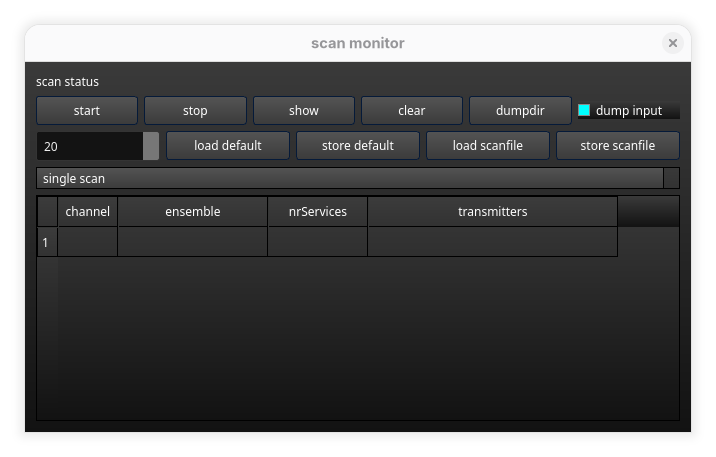
\includegraphics[width=90mm]{scan-controller.png}
\end{center}

The topline of the scan controller shows the status, when scanning it tells the
channel being visited.

The {\em scan mode} is set on the forth line. As mentioned above, the
mode is either {\em single scan}, i.e case 1 above, {\em until data}, i.e. case
2 above or {\em continuous}, i.e. case 3 above.
\par
It is often quite obvious that some channels are better skipped when
scanning, it is known that they do not contain DAB data.
Qt-DAB provides for that purpose so-called {\em scan files}.
A  scan file is a file containing a list of channels, where each channel
is marked whether it should be skipped or not.

\begin{center}
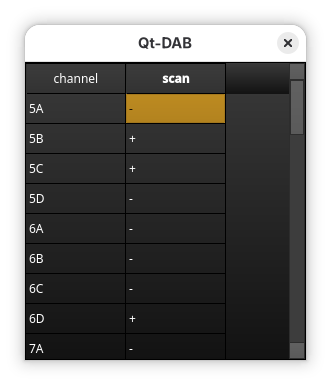
\includegraphics[width=60mm]{scanfile.png}
\end{center}

Two types of scan file are provided for:
\begin{enumerate}
\item a {\em default} one, the data of which is just recorded in the {\em .ini} file and
\item {\em named ones}, the data of which is stored into a file with a user defined name.
\end{enumerate}
The {\em third} line contains (from left to right):
\begin{enumerate}
\item a time indicator, telling the number of seconds to stay interpreting data in a selected channel (default 20 seconds);
\item the {\em load default} button, when touched the {\em default} scan list is shown (and can be manipulated);
\item the {\em store default} button, when touched the {\em default} scan list is stored (as the name suggests);
\item the {\em load scanfile} button, when touched a file selection
menu appears and {\em an existing} file can be selected;
\item the {\em store scanfile} button, when touched the content of the current scan list is  stored in a user defined scan file.
\end{enumerate}
Note that the regular way to create a user defined scan file is by:
\begin{enumerate}
\item loading the default scan file;
\item modifying it to your wishes, and
\item storing it as a user defined scan file.
\end{enumerate}

The scanlist itself is just a table with channel names, each with an indicator telling whether or not the channel should be visited when scanning.

The {\em second line} of the scan controller contains the actual control
buttons:
\begin{enumerate}
\item the {\em start} button starts the actual scanning, and
\item the {\em stop} button stops the scanning (obviously if scanning is on);
\item the {\em show} button shows the currently selected scanlist;
\item the {\em clear} button clears the scan list, i.e. all channels are visited;
\item the {\em dumpdir} button allows selection of a directory (folder) to storing the scan list(s);
\item the {\em dump input} button, when touched, causes the raw sample input from each channel to be written into a file, which is then written in ".csv" format.
\end{enumerate}
\section{Scan output}
\subsection{Single Scan}
The output of the scanner is split up into two parts:
\begin{enumerate}
\item in the scan control window, the channel where data was detected, together with the ensemble name, the number of services detected, and the transmitters detected with that channel is shown;
\item in a separate window, the details per channel are shown.
\end{enumerate}
\begin{center}
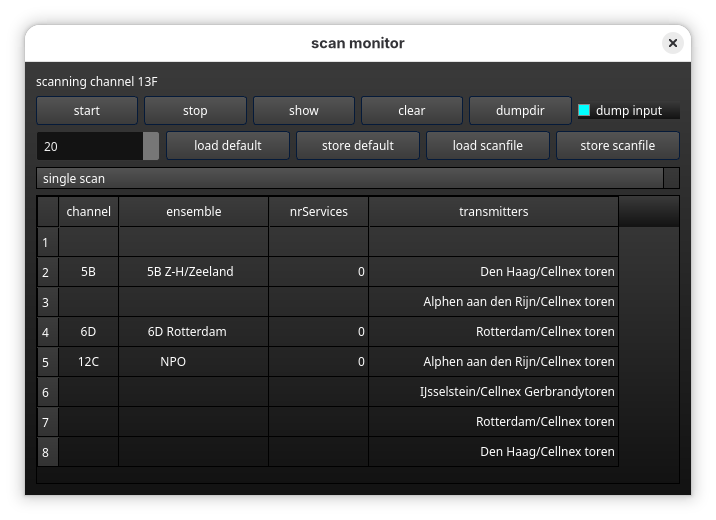
\includegraphics[width=90mm]{scanoutput-1.png}
\end{center}

Unfortunately, the number of services detected in the channels is not computed correctly, this will be fixed in a next version.
\begin{center}
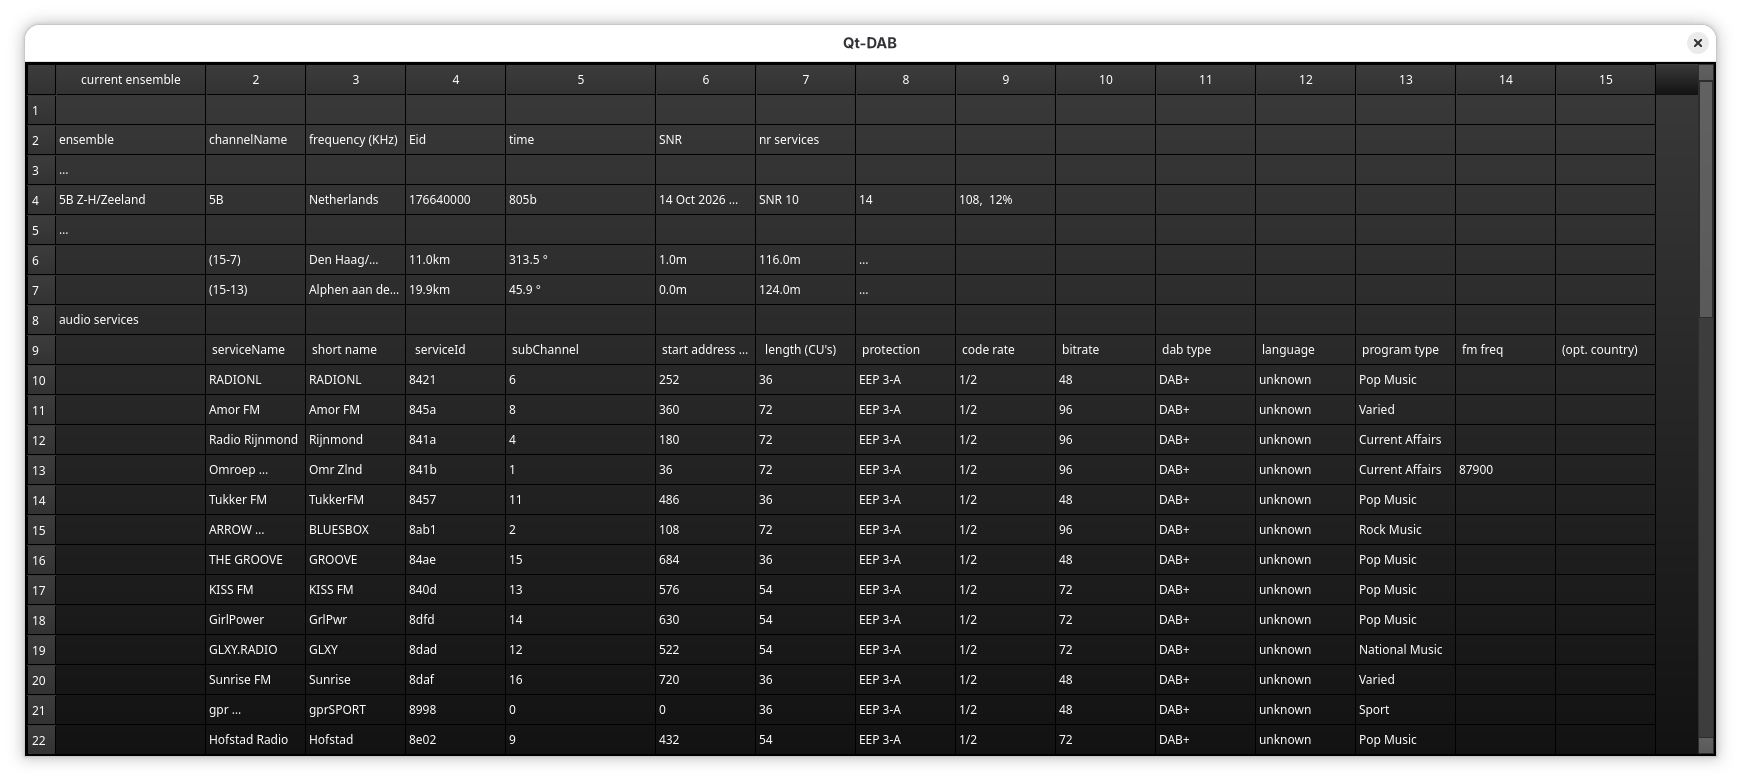
\includegraphics[width=150mm]{scanoutput-2.png}
\end{center}
As shown, the details of the ensemble detected in the channels are presented
in  the same format as used with the content dump of the current ensemble.
\par
At the end of the scan, one is asked whether or not contents description is
to be saved into a file in ".csv" format.
\begin{center}
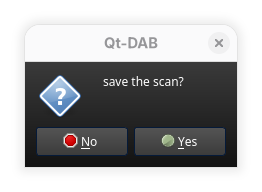
\includegraphics[width=50mm]{scanoutput-3.png}
\end{center}
\subsection{Scan to output}
Scan to output does not show output.
\subsection{Scan continuously}
When scanning continuously, the {\em per channel} data is somewhat limited
as no service names are shown.
The scan controller shows just the names of the ensembles detected
\begin{center}
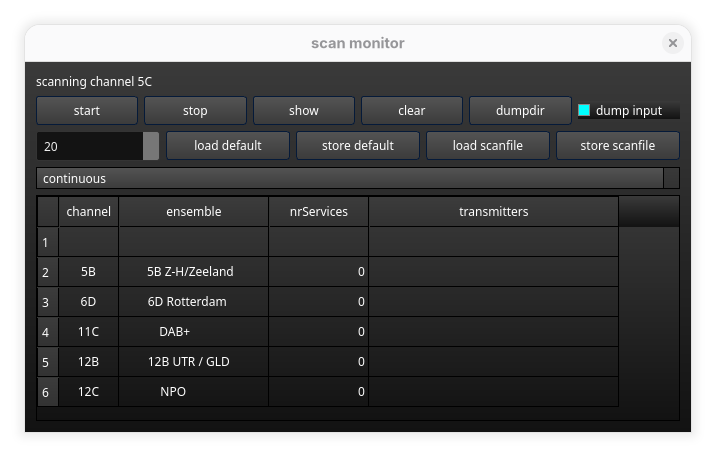
\includegraphics[width=90mm]{scanoutput-4.png}
\end{center}
A separate window gives per channel information in one or a few lines.
Note that the headings do not always match the content of the column, this
document describes the current version. It will be fixed in a next version
of Qt-DAB.
\begin{center}
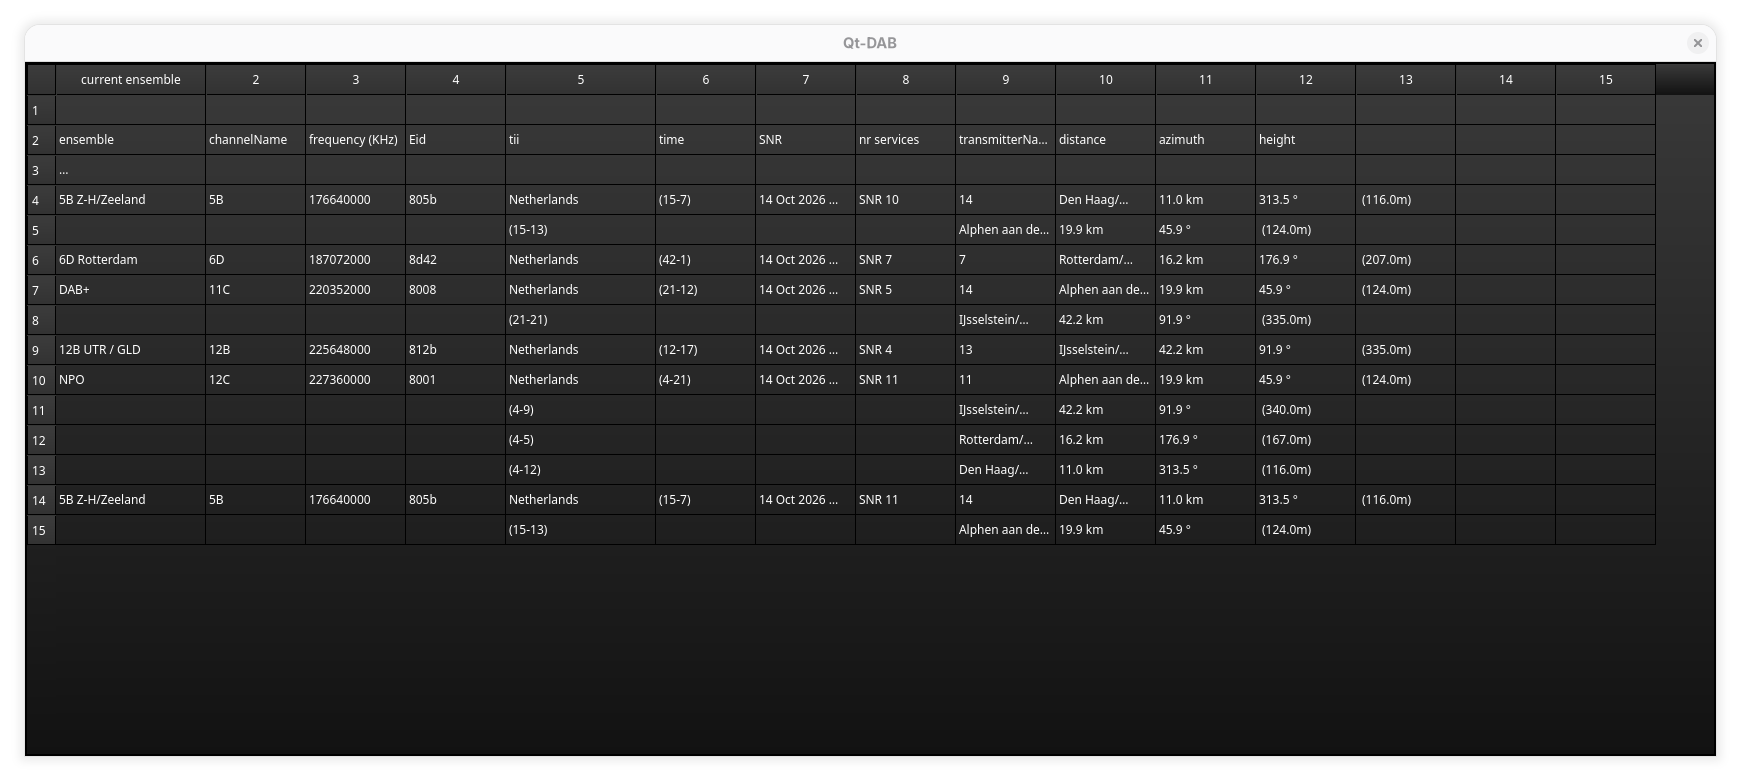
\includegraphics[width=150mm]{scanoutput-5.png}
\end{center}
Since the scanning continues, the common way of stopping the scan is by touching the {\em stop} button as mentioned above.
After having touched that button such that the scan stops,
one is asked whether or not to save the contents of the
separate window in a ".csv" type file.

\begin{center}
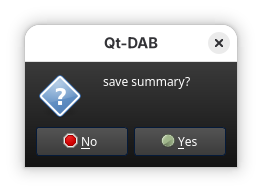
\includegraphics[width=55mm]{scanoutput-6.png}
\end{center}

\end{document}
